% @Author: Oscar Esteban
% @Date:   2015-02-20 15:40:09
% @Last Modified by:   Oscar Esteban
% @Last Modified time: 2015-03-26 17:57:06

\documentclass[a4paper]{report}

\usepackage{titlesec}
\newcommand{\sectionbreak}{\clearpage}

\usepackage{aliascnt}
\usepackage{relsize}
%\usepackage{inconsolata}
\usepackage[scaled]{beramono}
\usepackage[procnames]{listings}

\usepackage{natbib}
%\usepackage[style=numeric-comp,doi=false]{biblatex}

% *** GRAPHICS RELATED PACKAGES ***
\usepackage[table]{xcolor}
\usepackage{graphicx}
\usepackage{ifpdf}
\graphicspath{{figures/},{../Figures/}}

% *** MATH PACKAGES ***
\usepackage[cmex10]{amsmath}
\usepackage{amssymb}

\usepackage[T1]{fontenc}
\usepackage{charter}
%\usepackage[expert]{mathdesign}
%\usepackage[libertine,cmintegrals,cmbraces,vvarbb]{newtxmath}

% *** SPECIALIZED LIST PACKAGES ***
%\usepackage{algorithmic}
%\usepackage{algorithm}


% *** ALIGNMENT PACKAGES ***
%\usepackage{array}

% *** SUBFIGURE PACKAGES ***
\usepackage[font={small}]{caption}
%\usepackage{sidecap}

% *** FLOAT PACKAGES ***
\usepackage[framemethod=tikz]{mdframed}
%\usepackage{float}
% \usepackage{fixltx2e}
% \usepackage{stfloats}
% \usepackage{dblfloatfix}


% *** MISC UTILITY PACKAGES ***
%\usepackage{fancyhdr}
\usepackage{multicol}
\usepackage{tabularx}
\usepackage{longtable}
\usepackage{booktabs} % to use \toprule
\usepackage{makeidx}
%\usepackage[scale=2.0]{ccicons}
\usepackage[colorinlistoftodos]{todonotes}
\usepackage[top=2cm,bottom=1.8cm,left=2.1cm,right=1.7cm,marginparwidth=1.2in]{geometry}
\usepackage{changepage}
\usepackage{epigraph}
\usepackage[toc,nomain,acronym,shortcuts,translate=false]{glossaries}

\usepackage{mathtools}
\usepackage{amsmath}
\usepackage{amssymb}
\usepackage{cancel}
%\usepackage{algorithmic}
\DeclareMathOperator{\tr}{tr}
\DeclareMathOperator{\argmax}{argmax}
\DeclareMathOperator{\argmin}{argmin}
\DeclareMathOperator{\diag}{diag}
\DeclareMathOperator{\dist}{dist}
\DeclareMathOperator{\const}{Const.}
\providecommand{\e}[1]{\ensuremath{\times 10^{#1}}}
\providecommand{\mdist}[2]{ \mathcal{D}_{#2}^2(\mathbf{#1}) }
\let\oldhat\hat
\renewcommand{\vec}[1]{\mathbf{#1}}
\providecommand{\nvec}[1]{\hat{\mathbf{#1}}}

\renewcommand\thesection{S\arabic{section}}
\renewcommand\thesubsection{S\arabic{section}.\arabic{subsection}}
\renewcommand\thefigure{S\arabic{figure}}
\renewcommand{\theequation}{SM\arabic{equation}}

% Listings style -----------------------------------------------------------------------------
\definecolor{pink}{RGB}{255,0,90}
\definecolor{comments}{RGB}{50,120,110}
\definecolor{string}{RGB}{160,0,0}
\definecolor{keywords}{RGB}{0,150,0}
\definecolor{listingbg}{gray}{0.95}

\lstset{basicstyle=\ttfamily\smaller\relax}

\newcommand*{\codeinline}[1]{\colorbox{listingbg}{\lstinline!#1!}}
%\newcommand\codeinline{\lstinline}

\lstnewenvironment{bashcode}[1][]
  {\lstset{language={}}\lstset{%
  showstringspaces=false,
  formfeed=\newpage,
  tabsize=4,
  breaklines=true,
  basicstyle=\ttfamily\smaller\relax,
  keywordstyle=\color{keywords}\bfseries,
  commentstyle=\color{comments}\itshape,
  stringstyle=\color{string},
  showstringspaces=false,
  %identifierstyle=\color{green},
  morekeywords={regseg},
  numbers=none,
  frame=single,
  xleftmargin= 10pt,
  xrightmargin= 10pt,
  framexleftmargin=10pt,
  frameround=tttt,
  fillcolor=\color{listingbg},
  backgroundcolor=\color{listingbg}
}}
{}


\lstnewenvironment{pythoncode}[1][]
  {\lstset{language=bash}\lstset{%
  showstringspaces=false,
  formfeed=\newpage,
  tabsize=4,
  breaklines=true,
  basicstyle=\ttfamily\smaller\relax,
  keywordstyle=\color{keywords}\bfseries,
  commentstyle=\color{comments}\itshape,
  stringstyle=\color{string},
  showstringspaces=false,
  identifierstyle=\color{black!70},
  procnamekeys={def,class},
  morekeywords={models, lambda, forms, as, from, import},
  numbers=left,
  numberstyle=\smaller\color{black!60},
  stepnumber=1,
  numbersep=5pt,
  frame=single,
  xleftmargin= 40pt,
  xrightmargin= 20pt,
  framexleftmargin=20pt,
  frameround=tttt,
  fillcolor=\color{gray!10},
  backgroundcolor=\color{gray!10}
}}
{}

\usepackage[hyphens]{url}
\usepackage[hyphenbreaks]{breakurl} %fixes boxes spanning through pages
\usepackage[colorlinks=true,citecolor=blue,urlcolor=blue,linkcolor=blue]{hyperref}

% List of acronyms used in the text
\newacronym{mr}{MR}{magnetic resonance}
\newacronym{mri}{MRI}{magnetic resonance imaging}
\newacronym{dwi}{dMRI}{diffusion MRI}
\newacronym{dw}{DW}{diffusion weighted}
\newacronym{dti}{DTI}{diffusion tensor imaging}
\newacronym{t1}{T1}{T1-weighted}
\newacronym{t2}{T2}{T2-weighted}
\newacronym{csf}{CSF}{cerebrospinal fluid}
\newacronym{wm}{WM}{white matter}
\newacronym{gm}{GM}{grey matter}
\newacronym{epi}{EPI}{echo-planar imaging}
\newacronym{gre}{GRE}{gradient echo sequence}
\newacronym{fa}{FA}{fractional anisotropy}
\newacronym{md}{MD}{mean diffusivity}
\newacronym{acwe}{ACWE}{active contours without edges}
\newacronym{map}{MAP}{maximum a posteriori}
\newacronym{snr}{SNR}{signal-to-noise ratio}
\newacronym{pve}{PVE}{partial volume effect}
\newacronym{roi}{ROI}{region of interest}
\newacronym{mrf}{MRF}{Markov Random Field}

\newacronym{se}{SE}{Surface error}
\newacronym{wi}{WI}{Warping index}
\newacronym{nof}{NoF}{number of fibers}



\makeglossaries

%\acrodef{mr}[MR]{magnetic resonance}
%\acrodef{mri}[MRI]{magnetic resonance imaging}
%\acrodef{dwi}[DWI]{diffusion weighted imaging}
%\acrodef{dw}[DW]{diffusion weighted}
%\acrodef{dti}[DTI]{diffusion tensor imaging}
%\acrodef{t1}[T1]{T1-weighted}
%\acrodef{t2}[T2]{T2-weighted}
%\acrodef{csf}[CSF]{cerebrospinal fluid}
%\acrodef{wm}[WM]{white matter}
%\acrodef{gm}[GM]{grey matter}
%\acrodef{epi}[EPI]{echo-planar imaging}
%\acrodef{fa}[FA]{fractional anisotropy}
%\acrodef{md}[MD]{mean diffusivity}
%\acrodef{acwe}[ACWE]{active contours without edges}
%\acrodef{map}[MAP]{maximum a posteriori}
%\acrodef{snr}[SNR]{signal-to-noise ratio}
%\acrodef{pve}[PVE]{partial volume effect}
%\acrodef{roi}[ROI]{region of interest}


\begin{document}
\title{Supplemental Materials: \emph{Simultaneous segmentation and registration of
diffusion MR images of the brain driven by active-contours}}
\author{Oscar Esteban and Dominique Zosso}
\date{February 2015}

\maketitle
\section{Extensions to the mathematical formulation of the methods}

\subsection{Computing the gradients of shape-priors}\label{sec:shape_priors}
The computation of gradients at the locations of the active contours in the
  instant $t$ is based on the work of \cite{herbulot_segmentation_2006}.
Let $F(\vec{r})$ be an ``arbitrary'' function over the image domain
  $\Omega = \Omega_l \cup \Omega_m$ splitted in two regions $l$ and
  $m$, and $\Gamma_{l,m}$ a closed boundary between them.
We now derive the domain integral w.r.t. $t$:

  \begin{equation}
  \frac{\partial}{\partial t} \int_\Omega F(\vec{r}) d\vec{r} =
  \int_\Omega \frac{\partial}{\partial t}F(\vec{r}) d\vec{r} 
  - \int_{\Gamma_{l,m}} F(\vec{r}) \left\langle \frac{\partial \Gamma_{l,m} }{\partial t},
  N_{\Gamma_{l,m}}\right\rangle d\vec{r},
  \end{equation}
%
  where $\left\langle\frac{\partial\Gamma_{l,m}}{\partial t}, N_{\Gamma_{l,m}}\right\rangle$ is
  the projection of the boundary movement on the unit inward normal $N_{\Gamma_{l,m}}$.
Assuming that the region descriptors $\{\boldsymbol{\mu}_l, \boldsymbol{\Sigma}_l\}$ vary slowly enough, we can consider
  that $\frac{\partial}{\partial t} F(\vec{r}) = 0$ and thus:

  \begin{equation}
  \frac{\partial}{\partial t} \int_\Omega F(\vec{r}) d\vec{r} =
  - \int_{\Gamma_{l,m}} F(\vec{r}) \left\langle \frac{\partial \Gamma_{l,m} }{\partial t},
  N_{\Gamma_{l,m}}\right\rangle d\vec{r}.
  \label{eq:shape_gradients}
  \end{equation}

The equation \eqref{eq:shape_gradients} is discretized as follows.
First, the surface between limiting regions $\{l, m\}$, $\Gamma_{l,m}$ is explicitly represented by
  a discrete set of vertices $\vec{v}_i$, with $i \in \{0, \ldots, N_p -1 \}$.
Consequently, the inwards normal of the surface $N_{\Gamma_{l,m}}$ is represented by the discrete
  set of normals $\hat{\vec{n}}_i$ at each vertex of the mesh.
The resulting summation is, therefore, discrete and the integral operator is replaced by the sum:
  \begin{align}
  \frac{\partial}{\partial t} \int_\Omega F(\vec{r}) d\vec{r} &=
  \underbracket{\cancel{\int_\Omega \frac{\partial}{\partial t}F(\vec{r}) d\vec{r} }}_{\text{Functional's evolution}}
  - \underbracket{\int_{\Gamma_{l,m}} F(\vec{r}) \left\langle \frac{\partial \Gamma_{l,m}}{\partial t},
  N_{\Gamma_{l,m}}\right\rangle d\vec{r}}_{\text{Shape's evolution}} \notag \\
  & = - \underset{p}{\sum} \frac{1}{A_p} \underset{i}{\sum} \, a_i \, F(\vec{v}_i) \left\langle \underbracket{\frac{\partial \vec{v}_i}{\partial t}}_{\text{speed of }\vec{v}_i},
  \hat{\vec{n}}_{i}\right\rangle.
  \label{eq:shape_gradient_orig}
  \end{align}
where $a_i$ is the area corresponding to vertex $\vec{v}_i$, and $A_p = \sum_i a_i$ is the total area of surface $p$.
In the following, we will refer as $w_{p,i} = a_i / A_p $ to the area contribution of $\vec{v}_i$ to the
  total area of the surface it belongs to.
For simplicity, the sum over $p$ can be also removed, as the vertices belong to only one of the total $P$ contours

Then, the speed of $\vec{v}_i$ is discretized using the artificial time-step parameter $\delta$, as the displacement
  $\frac{\partial \vec{v}_i}{\partial t} = \vec{v}_i(\delta = t+1) - \vec{v}_i(\delta = t)$:
  \begin{equation}
  \frac{\partial}{\partial t} \int_\Omega F(\vec{r}) \, d\vec{r} =
  - \underset{i}{\sum} w_{p,i} F(\vec{v}_i) \frac{\partial \vec{v}_i}{\partial t} \cdot \hat{\vec{n}}_i.
  \label{eq:shape_gradient_disc1}
  \end{equation}

Since the energy functional is defined over competing regions, the displacement of $\vec{v}_i$ will cause
  an energy exchange between the limiting regions, and therefore $F(\vec{r})$ must be split in
  two terms, $F_{in}(\vec{r})$ corresponding to the interior region and $F_{out}(\vec{r})$ to the exterior:
  \begin{equation}
  \frac{\partial}{\partial t} \int_\Omega F(\vec{r}) \, d\vec{r} =
  - \underset{i}{\sum} \, \frac{\partial \vec{v}_i}{\partial t} \cdot
  \underbracket{w_{p,i} \, \Big[ F_{out}(\vec{v}_i) - F_{in}(\vec{v}_i) \Big] \hat{\vec{n}}_i}_{\bar{s}_i \text{ in Figure 1}}.
  \label{eq:shape_gradient_disc2}
  \end{equation}

\subsection{Gradient-descent optimization}\label{sec:gradient_descent}
The energy functional to be optimized
  in \emph{regseg} is presented in Eq. 7:
  \begin{equation}
  E(R \mid U) = C + \underbracket{\underset{l}{\sum} \int_{\Omega_l}
  \mdist{f'}{l} \,d\vec{r}}_{\text{Data term } (E_{data})}
  + \underbracket{\underset{\Omega}{\int} \left[ \boldsymbol{\alpha} \cdot \vec{u}^{\circ2}
  + \boldsymbol{\beta} \cdot (\nabla \vec{u})^{\circ2} \right] \,d\vec{r}}_{\text{Regularization term } (E_{reg})}.
  \label{eq:energy}
  \end{equation}

To search for the minimum of $E(R \mid U)$ w.r.t. the coefficients $\vec{u}_k$, we use a gradient descent strategy.
In Eq. 11 we introduced the derivative of \eqref{eq:energy}:
  \begin{equation}
  \frac{\partial E(\vec{u})}{\partial \vec{u}_k} =
  \frac{ \partial }{\partial \vec{u}_k} \Big\{
  \underset{l}{\sum} \int_{\Omega_l} \mdist{f'}{l} \,d\vec{r}
  + \int_{\Omega} \frac12 [ \boldsymbol{\alpha} \cdot \vec{u}^{\circ2}
  + \boldsymbol{\beta} \cdot (\nabla \vec{u})^{\circ2} ] \,d\vec{r}
  \Big\}.
  \label{eq:gradient_descent}
  \end{equation}

We split \eqref{eq:gradient_descent} in the derivatives of its data and regularization terms.
Let $\frac{\partial E_{data}}{\partial \vec{u}_k} = \vec{g}_k$ for simplicity, 
  we compute the derivative of the data term and discretize the domain $\Omega$ as follows:
\begin{equation}
  \vec{g}_k =
  \frac{ \partial }{\partial \vec{u}_k} \Big\{
  \underset{l}{\sum} \int_{\Omega_l} \mdist{f'}{l} \Big\} =
  \frac{ \partial }{\partial \vec{u}_k} \Big\{ \underset{l}{\sum} \underset{\vec{x} \in \Omega_l}{\sum} \, \mdist{f'}{l} \Big\},
  \label{eq:data_derivative}
\end{equation}
  where we can apply the shape-gradients \eqref{eq:shape_gradient_disc2} introduced
  in \autoref{sec:shape_priors}, and ultimately avoid implementing level sets:

  \begin{align}
  \vec{g}_k &= \underset{i}{\sum} \left\langle \frac{\partial \vec{v}_i'}{\partial \vec{u}_k}, \bar{s}_i'\right\rangle, \\
  \text{with }
  \bar{s}_i' &= - w_i \left[ \mdist{f_i'}{out} - \mdist{f_i'}{in} \right] \, \hat{\vec{n}}_i, \\
  \text{and } 
  \frac{\partial \vec{v}_i'}{\partial \vec{u}_k} &=
  \frac{\partial}{\partial \vec{u}_k} \left\{ \vec{v}_i + \sum_k \psi_k(\vec{v}_i) \vec{u}_k \right\} = \psi_k(\vec{v}_i)\, \hat{\vec{e}}.
  \label{eq:gradient_wshape}
  \end{align}%
  where $\hat{\vec{e}}$ is the coordinates system's unit vector.
Therefore, the shape gradients projected to the grid of B-Spline control points is:
\begin{equation}
  \vec{g}_k =
  - \underset{i}{\sum} \bar{s}_i \cdot \psi_k(\vec{v}_i) \, \hat{\vec{e}} = - \underset{i}{\sum} \vec{g}_{i,k}.
  \label{eq:shape_gradient_final}
\end{equation}

It is also necessary to obtain and discretize the derivatives of the regularization term of \eqref{eq:gradient_descent}:
  \begin{equation}
  \frac{\partial E_{reg}(\vec{u})}{\partial \vec{u}_k} = \frac{ \partial }{\partial \vec{u}_k} \Big\{
  \int_{\Omega} \frac12 [ \boldsymbol{\alpha} \cdot \vec{u}^{\circ2}
  + \boldsymbol{\beta} \cdot (\nabla \vec{u})^{\circ2} ] \,d\vec{r}
  \Big\} = \boldsymbol{\alpha} \cdot \vec{u}_k + \boldsymbol{\beta} \cdot \Delta \vec{u}_k.
  \label{eq:gradient_regterm}
  \end{equation}

Inserting \eqref{eq:shape_gradient_final} and \eqref{eq:gradient_regterm} into \eqref{eq:gradient_descent} we get the
  final evolution equation:
  \begin{equation}
  \frac{\partial E(\vec{u})}{\partial \vec{u}_k} = \vec{g}_k + \boldsymbol{\alpha} \cdot \vec{u}_k + \boldsymbol{\beta} \cdot \Delta \vec{u}_k,
  \label{eq:gradient_final}
  \end{equation}


\subsection{Obtaining the update equation} To solve the differential equation in \eqref{eq:gradient_descent},
  we use a semi-implicit Euler scheme, referring to the discrete step size as $\delta$ and where the
  shape-gradients $\vec{g}_k$ are explicit:
\begin{align}
  \vec{u}_k^{t+1} &= \vec{u}_k^{t} + \delta \, \Big( \vec{g}_k^{t+1} + (\boldsymbol{\alpha} - \boldsymbol{\beta} \Delta) \, \vec{u}_k^{t+1} \Big) \notag \\
  (1 - \delta \boldsymbol{\alpha} - \delta \boldsymbol{\beta} \Delta)\, \vec{u}_k^{t+1} &= \vec{u}_k^{t} + \delta\, \vec{g}_k^{t}
  \label{eq:discrete_derivative}
\end{align}

This expression is easily translated into Fourier domain as follows:

  \begin{align}
  \vec{u}_k^{t+1} = \mathcal{F}^{-1}\left\{ \frac{\mathcal{F}\{\delta^{-1} \, \vec{u}_k^t + \vec{g}_k\} }%
                  {\mathcal{F}\{(\delta^{-1} - \boldsymbol{\alpha})\, I-\boldsymbol{\beta}\Delta\}} \right\},
  \label{eq:update_equation}
  \end{align}
  where $I$ denotes the identity operator.
Here, we rewrite the Laplacian as a linear combination of the identity and shift operators:
  \begin{equation}
  \Delta = \{\sum_{d=1}^n \mathcal{S}_d^- + \mathcal{S}_d^+\}  - 2n \mathcal{I}
  \end{equation}
  where $\mathcal{S}_d^{\pm}$ stands for the forward ($+$) and backward ($-$) shift operator along axis $d$, of which the Fourier transform is found easily as
  \begin{equation}
  \mathcal{F}\{\mathcal{S}_d^{\pm}\} = e^{\pm i\omega_d},
  \end{equation}
  where $\omega_d$ is the normalized pulsation along direction $d$.
Accordingly, the Fourier transform of the discrete Laplacian is found as
  \begin{align}
  \mathcal{F}\{\Delta\} &= \sum_d e^{-i\omega_d} + e^{i\omega_d} - 2n = n \, \left( \sum_d \cos(\omega_d) - 2\, \right)
  \end{align}

The remaining transforms are trivial or can be computed using FFT as in \citep{estellers_efficient_2012}.

%Then, introducing \eqref{eq:intp_kernel} into \eqref{eq:nodes_tfm} and replacing
%  $\psi$ by the actual kernel function, the transformation writes:
%
%  \begin{equation}
%    \vec{v}_i' = \vec{v}_i + \sum_k \left[ \vec{u}_k \, \underset{d}{\prod}
%      \beta_3( (\vec{v}_i - \vec{r}_k) \cdot \hat{\mathbf{e}}_d ) \right],
%  \label{eq:transformation}
%  \end{equation}
%%
%  with $\hat{\mathbf{e}}_d$ being the unitary vector along axis $d$.

\section{Parameter settings and implementation details of \emph{regseg}}

\subsection{Implementation}
\subsection{General} The \emph{regseg} registration and segmentation tool is written in C++, using ITK-4.6 as
  implementation core.
We designed a modular implementation, enabling multithreading in several pieces of the software,
  as the process is computationally expensive.
The tool generates a log-file in JSON format to easily inter-operate with secondary tools (such
  as the convergence report generation, \autoref{sec:convergence_evidence}).

\subsection{Efficient interpolation using sparse matrices}
During the registration process, every iteration requires computing the product of all the gradients
  $\vec{g}_k$ associated to the control point $k$, and computed at the current position
  $\vec{v}_i$ by the corresponding weights $\psi_{ik} = \psi_k(\mathbf{v}_i)$ of interpolating functions
  \eqref{eq:shape_gradient_final}.
In order to optimize multiplications and summations, all the $\psi_{ik}$ are collected in a
  matrix $\boldsymbol{\Psi} = (\psi_{ik})$.
Given the limited support of the basis function $\psi$, $\boldsymbol{\Psi}$ will hold the property
  of being sparse, as only few $\psi_{ik} > 0$ in the surroundings of $\vec{v}_i$.
Then, the gradients $\vec{g}_k$ are easily computed using the matrix product:
\begin{equation}
  \big(\vec{g}_k \big) = \boldsymbol{\Psi} \cdot \big( w_i \, \bar{s}_i \big)^T
  \label{eq:sparse_matrix}
\end{equation}

As these weights can be computed once in the beginning of the process and they do not change along
  it, $\boldsymbol{\Psi}$ can be pre-cached.

\subsection{Interface and Settings}\label{sec:interface_settings}

\paragraph{Command-line interface}
The command line interface of \emph{regseg} supports general settings and level-wise settings.
For each multi-resolution level, its corresponding settings are added between brackets.

\begin{bashcode}
regseg -F fa.gz adc.nii.gz -P white.vtk pial.vtk -o myprefix [ -a 0.00000 -b 0.00000 --convergence-energy -t 1.0e-06 -w 60 --adaptative-descriptors --grid-spacing 16.0 -i 500 -s 0.001] [ -a 0. -b 0. --convergence-energy -t 1.e-08 -w 5 --grid-spacing 8.0 -i 250 -s 0.01]
\end{bashcode}


It is possible to get the description of available options running
  \codeinline{regseg -h}:

\begin{bashcode}
Usage:

General options:
  -h [ --help ]                         show help message
  -F [ --fixed-images ] arg             fixed image file
  -P [ --surface-priors ] arg           shape priors
  -T [ --surface-target ] arg           final shapes to evaluate metric (only
                                        testing purposes)
  -M [ --fixed-mask ] arg               fixed image mask
  -L [ --transform-levels ] arg         number of multi-resolution levels for
                                        the transform
  -o [ --output-prefix ] arg (=regseg)  prefix for output files
  -l [ --logfile ] arg                  log filename
  -v [ --monitoring-verbosity ] arg (=1)
                                        verbosity level of intermediate results
                                        monitoring ( 0 = no output; 5 = verbose
                                        )

Optimizer options (by levels):
  -a [ --alpha ] arg              alpha value in regularization
  -b [ --beta ] arg               beta value in regularization
  -s [ --step-size ] arg          step-size value in optimization
  -g [ --gradient-scales ] arg    alpha value in regularization
  -r [ --learning-rate ] arg      learning rate to update step size
  -i [ --iterations ] arg         number of iterations
  -w [ --convergence-window ] arg number of iterations of convergence window
  -t [ --convergence-thresh ] arg convergence value
  --grid-size arg                 size of control points grid
  --grid-spacing arg              spacing between control points
  -u [ --update-descriptors ] arg frequency (iterations) to update descriptors
                                  of regions (0=no update)
  --adaptative-descriptors        recomputes descriptors more often at the
                                  beginning of the process
  --convergence-energy            disables lazy convergence tracking: instead
                                  of fast computation of the mean norm of the
                                  displacement field, it computes the full
                                  energy functional

Functional options (by levels):
  --smoothing arg               apply isotropic smoothing filter on target
                                image, with kernel sigma=S mm.
  --smooth-auto                 apply isotropic smoothing filter on target
                                image, with automatic computation of kernel
                                sigma.
  --uniform-bg-membership       consider last ROI as background and do not
                                compute descriptors.
  -d [ --decile-threshold ] arg set (decile) threshold to consider a computed
                                gradient as outlier (ranges 0.0-0.5)

\end{bashcode}

\paragraph{\emph{Nipype} interface}
Our registration algorithm is released with a \emph{nipype Interface} packaged in
  \codeinline{pyacwereg.interfaces.acwereg}.
This interface has been comprehensively used in the evaluation workflows.

\begin{pythoncode}
from pyacwereg.interfaces.acwereg import ACWEReg
regseg = ACWEReg()
regseg.inputs.in_fixed = ['T1w.nii.gz', 'T2w.nii.gz']
regseg.inputs.in_pior = ['csf.vtk', 'white_lh.vtk', 'white_rh.vtk',
                         'pial_lh.vtk', 'pial_rh.vtk']
ifresult = regseg.run()
\end{pythoncode}


\subsection{Convergence evidencing}\label{sec:convergence_evidence}

In order to track the evolution of the registration process, several internal variables
  are saved in the JSON log-file.
Using the JSON log-file as input for the \emph{nipype Interface}
  \codeinline{ACWEReport}, it is straightforward to obtain
  a visual assessment document presenting the convergence.
\begin{pythoncode}
from pyacwereg.interfaces.acwereg import ACWEReport
report = ACWEReport()
report.inputs.in_log = `myprefix.log'
ifresult = report.run()
\end{pythoncode}

Online checking is also possible as the algorithm writes to the standard output as well.
A sample report is found in \autoref{fig:convreport}.

\begin{figure*}[b]
  \includegraphics[width=\textwidth]{figures/Suppl-figure02.pdf}
  \caption{The evolution of the registration and segmentation process can be
    checked using the \emph{Convergence report},
    easily generated using the appropriate \emph{nipype Interface}.
  The report comprehends several plots tracking the evolution of the algorithm and several
    features to help researchers tune up the algorithm in their application.}%
    \label{fig:convreport}
\end{figure*}

\section{Instruments for evaluation}

This work is supported by two \emph{nipype Workflows} in order to ensure the reproducibility
  of the results.
All the intermediate results and figures in this paper have been encapsulated into
  the workflows and are available in \url{http://dx.doi.org/zenodolink}.

An overview of the general workflow is presented in the Figure 2 of the paper.
However, this figure has been extremely simplified for the best of visualization.
In this section, we review the main elements of the evaluation pipelines.

\subsection{Assessment of the segmentation model}
\begin{figure}
  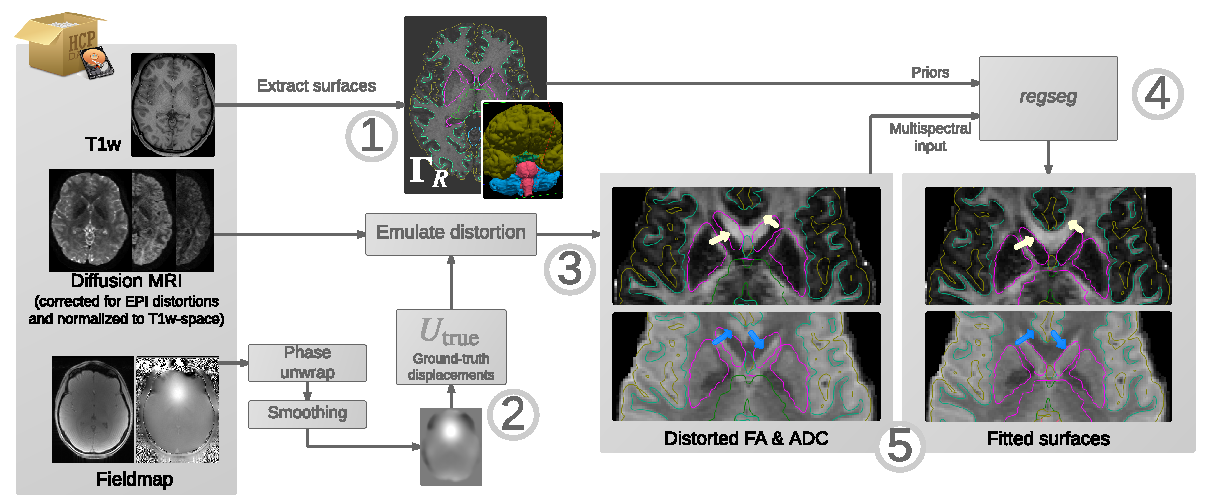
\includegraphics[width=\linewidth]{figures/figure04.pdf}
  \caption{Assessment of the segmentation model, sampling the value of the energy functional
  \eqref{eq:energy} versus several registration errors generated as explained in
  \autoref{sec:res_model_and_metric}.
  The metric of our registration method displayed a smooth gradient towards the minimum
  located at the $\epsilon = 0.0$ point.}\label{fig:energymap}
\end{figure}


\subsection{Preprocessing}

\subsection{Distortion}

\section{Model considerations}

\begin{figure*}[!ht]
	\includegraphics[width=\textwidth]{figures/Suppl-figure01.pdf}
	\caption{Evaluating the joint distribution}\label{fig:jointplot}
\end{figure*}

\newpage
\section{Extended results on real data}

\immediate\write18{./visual_report.sh}
\input{suppl-realdata.tex}

\bibliographystyle{mystyle}
\bibliography{Remote}

\end{document}




%{\color{red} {The main diverging points with respect to
%\citep{gorthi_active_2011} are: 1) there is no need for an explicit level set function
%$\Phi_G$, as we replace the level set gradient computation $N_{\Phi_G}$ with shape
%gradients \citep{besson_dream2s_2003,herbulot_segmentation_2006};
%2) regularization is also based on linear diffusion smoothing \citep{thirion_image_1998},
%but we replace the Gaussian filtering by other constraints
%studied in \citep{nagel_investigation_1986} to better the problem;
%3) optimization is applied in the spectral
%domain, observing anisotropic and inhomogeneous mappings along each direction.
%With respect \citep{guyader_combined_2011}, the main differences are
%the distance function, and the spectral solution to the optimization updates,
%as we shall cover in \autoref{sec:numerical_implementation}.}}



%In this paper we formulate the joint registration-segmentation
%problem as follows.
%such that the known contours in anatomical space $T$ optimally segment
%the diffusion space $D$.
%
%
%Whereas related \glspl*{adf} introduced in \autoref{sec:methods_background}
%make use of explicit level-set formulations to solve \eqref{eq:gradient_descent},
%we alternatively use \emph{shape-gradients}
%\cite{besson_dream2s_2003,herbulot_segmentation_2006}.

%
%Let us denote by $\vec{x}$ the voxel and $F(\vec{x}) = [ f_1, f_2, \ldots, f_N]^T$
%  its associated feature vector in the following.
%
%In our application, these surfaces are precise tissue interfaces of interest extracted
%  from a high-resolution, anatomically correct reference volume using
%  the well-established
%
%In this paper we propose a novel registration framework to simultaneously
%solving the segmentation, distortion and cortical parcellation challenges,
%by exploiting as strong shape-prior the detailed morphology extracted
%from high-resolution and anatomically correct \gls{mri}.
%Indeed, hereafter
%we assume this segmentation problem in anatomical images is reliably and
%accurately solved with readily available tools (e.g.
%\citep{fischl_freesurfer_2012}).
%After global alignment with \gls{t1} using existing approaches, the remaining
%spatial mismatch between anatomical and diffusion space is due to susceptibility
%distortions.
%Finally, we need to establish precise spatial correspondence between the
%surfaces in both spaces, including the tangential direction for parcellation.
%Therefore, we can reduce the problem to finding the differences of spatial
%distortion in between anatomical and \gls{dwi} space.
%We thus reformulate the segmentation problem as an inverse problem, where we
%seek for an underlying deformation field (the distortion) mapping
%from the structural space into the diffusion space, such that the structural
%contours segment optimally the \gls{dwi} data.
%In the process, the one-to-one
%correspondence between the contours in both spaces is guaranteed, and projection
%of parcellisation to \gls{dwi} space is implicit and consistent.
%
%We test our proposed joint segmentation-registration model on two different
%synthetic examples.
%The first example is a scalar sulcus model, where the
%\gls{csf}-\gls{gm} boundary particularly suffers from \gls{pve} and can only be
%segmented correctly thanks to the shape prior and its coupling with the inner,
%\gls{gm}-\gls{wm} boundary through the imposed deformation field regularity.
%The second case deals with more realistic \gls{dwi} data stemming from
%phantom simulations of a simplistic brain data.
%Again, we show that the
%proposed model successfully segments the \gls{dwi} data based on two derived
%scalar features, namely \gls{fa} and \gls{md}, while establishing an estimate
%of the dense distortion field.
%
%The rest of this paper is organized as follows.
%First, in \autoref{sec:methods}
%we introduce our proposed model for joint multivariate segmentation-registration.
%Then we provide a more detailed description of the data and experimental setup in
%\autoref{sec:experiments}.
%We present results in \autoref{sec:results} and conclude
%in \autoref{sec:conclusion}.
%
%
%The properties of the reconstructed tensors and derived scalar maps have
%been studied by \cite{ennis_orthogonal_2006}. Based on their
%findings, \gls{fa}~\eqref{eq:fa} and \gls{md}~\eqref{eq:md} are
%considered complementary features, and therefore we selected them for the
%energy model \eqref{eq:complete_energy} in driving the
%registration-segmentation process.
%Whereas \gls{fa} informs mainly about the \emph{shape} of diffusion,
%the \gls{md} is more related to the \emph{magnitude} of the process:
%
%\begin{align}
%\mathrm{FA} &= \sqrt{ \frac{1}{2}}\,\frac{\sqrt{ (\lambda_1 - \lambda_2)^2 + (\lambda_2 - \lambda_3)^2 + (\lambda_3 - \lambda_1)^2}}{\sqrt{ {\lambda_1}^2 + {\lambda_2}^2 + {\lambda_3}^2}} \label{eq:fa} \\
%\mathrm{MD} &= ( \lambda_1 + \lambda_2 + \lambda_3 ) / 3 \label{eq:md}
%\end{align}
%where $\lambda_i$ are the eigenvalues of the diffusion tensor
%associated with the diffusion signal $S(\vec{q})$. There exist
%two main reasons to justify their choice.
%First, they are well-understood and standardized in clinical routine.
%Second, together they contain most of the information that is
%usually extracted from the \gls{dwi}-derived scalar maps
%\cite{ennis_orthogonal_2006}.
%